\documentclass[a4paper,12pt]{article}
\usepackage{package}
%\usepackage[default]{gillius}
\usepackage[sfdefault,scaled=.85]{FiraSans}
\usepackage{newtxsf}
\usepackage{geometry}



%customization
\newgeometry{margin=0.75in,includefoot}
\setlength{\headheight}{14.49998pt}
\setlength{\footskip}{14.49998pt}



%Custom Theorem Environment
\usetikzlibrary{calc}
\tcbuselibrary{skins}
\usepackage{xcolor}
\usetikzlibrary{ shapes.geometric }
\usetikzlibrary{calc}


\definecolor{titleboxcolor}{RGB}{75, 204, 49}

\newcommand{\titlepath}{
  \fill[titleboxcolor]
  (title.south east)
  --(title.east)coordinate(A)
  to[curve to,out=90,in=0]($(A)+(-5mm,5mm)$)
      --($(title.north west)+(5mm,0mm)$)coordinate(B)
to[curve to,out=180,in=90]($(B)+(-5mm,-5mm)$)coordinate(C)
      --($(C)+(0mm,-5mm)$)
      to[curve to,out=90,in=180]($(title.south west)+(+5mm,0mm)$)coordinate(F)
      --cycle;
      \draw[titleboxcolor,ultra thick]
      ([yshift=.5\pgflinewidth]title.south east)--
      ([yshift=.5\pgflinewidth]title.south-|interior.east);
    }

\newtcolorbox{headBox}[1]{
    enhanced,
    frame empty,
    title= #1, %Name of the title
    colback=black!5,
    coltitle=white,
    attach boxed title to top left={xshift=-5mm},
    boxed title style={empty},
    underlay boxed title=\titlepath
    
}

%Theorem environment without Theorem name
\newtheorem{theorem}{}
\newtheorem{proposition}{}
\newtheorem{lemma}{}
\newtheorem{defination}{}

\theoremstyle{definition}
\newtheorem{example}{Example}[section]

%New Q and Ans environment
\newcommand\QQ[2]{\par\noindent \textbf{Q{#1}} {\itshape\textcolor{red}{#2}}\par \vspace{5pt}}
\newcommand\Ans[1]{\par\noindent \textbf{\textit{Ans:}} {{#1}}\par \vspace{10pt}}




%basic information
\title{GT}
\author{Abhi Mondal}
\date{\today}

\begin{document}
%Paragraph
%\setlength{\parindent}{20pt}
%title
\begin{center}
    
\includegraphics[scale = 0.075]{images/logos/R.png}\\
    \vspace{5pt}
    \textbf{\LARGE{Group Theory}}\\
    \vspace{10pt}
    \fontfamily{qhv}\selectfont{\textbf{By Abhi Mondal}} \\
\end{center}
\vspace{10pt}

\begin{headBox}{Source}
    Group Theory for Physicists with Applications by \emph{Pichai Ramadevi and Varun Dubey}
\end{headBox}

\begin{myquote}[red]
    \textbf{Keywords}: Group theory, Symmetry groups, Cyclic groups, Conjugacy class
\end{myquote}
\tableofcontents

\section{Motivation}

The group theory help us to exploit the symmetry without directly solving the differential equation explicitly. But the physicists are not that lazy! They are more curious to know the nature more intuitively!

\begin{itemize}
    \item 1-D Harmonic Oscillator $\rightarrow$ $SO(2)$ symmetry
    \item Hydrogen atom $\rightarrow$ Spherical symmetry
    \item Electrons in atom $\rightarrow$ Permutation symmetry
\end{itemize}

\noindent\textbf{Discrete Groups}
Cyclic group, Permutation group, point group, Irreducible representations, Character tables and applications in solid state physics.
\newline
\textbf{Continuous Groups}
Space-time symmetry, translational symmetry, rotational symmetry.
Examples: $SU(2)$, $SU(3)$ (covering group applications).

\[
\begin{aligned}
\text{Rotation of Square} \qquad & \text{Rotation of Circle} \\
\downarrow \qquad \qquad & \qquad \downarrow \\
\text{Discrete} \qquad & \text{Continuum}
\end{aligned}
\]
We can write for Square by $\{ I, R_{\pi/2}, R_{\pi}, R_{3\pi/2} \}$  while for Circle, we need rotation by any angle $\theta$ which is \imp{continuous}. The rotation group of a circle is Abelian. 

\section{Group}

A set $G = \{a,b,c,\dots\}$ with a binary operation $\cdot$
is called a group if:

\begin{enumerate}
    \item Closure: $a \cdot b \in G$
    \item Associativity: $(a \cdot b) \cdot c = a \cdot (b \cdot c)$
    \item Identity element: $\exists e \in G$ such that $ae = ea = a$
    \item Inverse: $\forall a \in G$, $\exists a^{-1} \in G$ such that $aa^{-1} = a^{-1}a = e$
\end{enumerate}

\subsection{Examples}

\begin{enumerate}
    \item $\mathbb{R}$ under addition is an Abelian group.
    \item $\mathbb{Z}$ under addition is an Abelian group.
    \item $\mathbb{R} - \{0\}$ under multiplication is Abelian.
    \item The set of all $2 \times 2$ matrices under matrix multiplication 
          is not Abelian in general.
\end{enumerate}

\begin{enlight}[green]{\bulb}
    \tcblower
    If for any group G with $a,b \in G$
    \[
    a \cdot b = b \cdot a
    \]
    then $G$ is called an \imp{Abelian group}.
\end{enlight}

\subsection{Subgroup}

If $H \subseteq G$ and $H$ itself satisfies group properties under
the same operation, then $H$ is called a subgroup of $G$. In notation we can write $H \leq G$.

\section{Basics of Groups' Properties}
\subsection{Multiplication Table}

A multiplication table helps verify closure and understand the structure of a finite group.
\newline
\textbf{Example}: Consider the rotation group of a square
\[
G = \{ e, R_{\pi/2}, R_{\pi}, R_{3\pi/2} \}
\]

\[
\begin{array}{c|cccc}
 & e & R_{\pi/2} & R_{\pi} & R_{3\pi/2} \\
\hline
e & e & R_{\pi/2} & R_{\pi} & R_{3\pi/2} \\
R_{\pi/2} & R_{\pi/2} & R_{\pi} & R_{3\pi/2} & e \\
R_{\pi} & R_{\pi} & R_{3\pi/2} & e & R_{\pi/2} \\
R_{3\pi/2} & R_{3\pi/2} & e & R_{\pi/2} & R_{\pi}
\end{array}
\]


\subsection{Order of a Group}

The number of elements in $G$ is called the \textbf{order} of $G$,
denoted by $|G|$. For the above example:
\[
|G| = 4
\]
A group with finite number of elements is called a \textbf{finite group}.

\subsection{Generator Set}
A subset $S$ of elements of a group $G$ is said to generate $G$ if every
element of $G$ can be expressed as a finite product of finite powers of elements (or
their inverses) of $S$ in some order. For \emph{finite} $S$, the elements of the minimal set $S$ that generates a group $G$ are called the \imp{generators} of the group and $S$ itself is called the \emph{generating set}.

A group whose generating set contains a \emph{single element} is said to be a \imp{cyclic group}.

\begin{example}
    Cyclic Group $C_n$ 
    with $a^n = e$
    \[
    C_n = \{ e, a, a^2, \dots, a^{n-1} \}
    \]
    The order of each element divides $n$.
\end{example}

\begin{example}
    $C_3$ with $a^3 = e$
    \[
    C_3 = \{ e, a, a^2 \}
    \]
    Multiplication table:

    \[
    \begin{array}{c|ccc}
    & e & a & a^2 \\
    \hline
    e & e & a & a^2 \\
    a & a & a^2 & e \\
    a^2 & a^2 & e & a
    \end{array}
    \]

\end{example}

\begin{example}
    The \emph{Klein group} $V_4$ has elements with generator set $\{a, b\}$ :

    \[
    V_4 = \{ e, a, b, ab \}
    \]
    with properties:
    \[
    a^2 = b^2 = e, \quad ab = ba
    \]
    It is Abelian group but not cyclic.
\end{example}

\begin{example}
    
Consider a group of a generator set $\{a, b\}$ with the following relations :
\[
a^3 = e,
\qquad
b^2 = e,
\qquad
ab = b^{2}a
\]
The group elements are:
\[
G = \{ e, a, a^2, b, ab, a^2b \}
\]
This is a \emph{non-Abelian} group of order 6. We denoted this group with $\mathfrak{S}(3)$ and called it \imp{Symmetric Group}.
\newline
Multiplication Table:

\[
\begin{array}{c|cccccc}
\mathfrak{S}(3) & e & a & b & b^2 & ab & ab^2 \\ \hline
e & e & a & b & b^2 & ab & ab^2 \\ 
a & a & e & ab & ab^2 & b & b^2 \\ 
b & b & ab^2 & b^2 & e & a & ab \\ 
b^2 & b^2 & ab & e & b & ab^2 & a \\ 
ab & ab & b^2 & ab^2 & a & e & b \\ 
ab^2 & ab^2 & b & a & ab & b^2 & e 
\end{array}
\]
\end{example}

\subsection{Example of a Non-Abelian Structure}

Consider a group with relations:
\[
a^2 = e, \qquad b^2 = e
\]
but
\[
ab \neq ba.
\]
In such a case, the elements can be:
\[
G = \{ e, a, b, ab, ba, aba, bab, \dots \}
\]
The multiplication is determined by the defining relations.

\subsection{Cosets}
Let $G$ be a group and $H \leq G$ a subgroup. For any $a \in G$, the \textit{left coset} of $H$ determined by $a$ is
\begin{equation*}
aH = \{ ah \mid h \in H \}.
\end{equation*}
Thus, we fix $a$ and multiply it with every element of $H$. Since the identity element $e \in H$, we have
\begin{equation*}
a = ae \in aH,
\end{equation*}
Similarly we have \emph{right coset}

\subsection{Equality of Cosets}

Suppose $aH$ and $bH$ have a common element. Then there exist $h_1, h_2 \in H$ such that
\begin{equation*}
ah_1 = bh_2.
\end{equation*}
Multiplying on the left by $a^{-1}$ gives
\begin{equation*}
a^{-1}b = h_1 h_2^{-1}.
\end{equation*}
Since $H$ is a subgroup, $h_1 h_2^{-1} \in H$, hence
\begin{equation*}
a^{-1}b \in H.
\end{equation*}
Conversely, if $a^{-1}b \in H$, then $b = ah$ for some $h \in H$, and therefore
\begin{equation*}
bH = aH.
\end{equation*}
Thus,
\begin{equation*}
aH = bH \quad \Longleftrightarrow \quad a^{-1}b \in H.
\end{equation*}
\imp{Hence two cosets are either identical or disjoint.}

\subsection{Cosets Partition the Group}

Every element $g \in G$ belongs to the coset $gH$. If $g \in aH$, then $g = ah$ for some $h \in H$. Therefore, the cosets are disjoint and their union equals $G$:

\begin{equation*}
G = \bigcup_{a \in G} aH.
\end{equation*}
So the cosets of $H$ form a partition of $G$.

\subsection{Size of a Coset}

Define the map
\begin{equation*}
\phi : H \to aH, \qquad \phi(h) = ah.
\end{equation*}
This map is bijective. Hence,
\begin{equation*}
|aH| = |H|.
\end{equation*}
\emph{Thus every coset has exactly the same number of elements as $H$.}

\begin{stkynote}[green]{Lagrange's Theorem}

    If $G$ is finite and $H \leq G$, then $G$ is a disjoint union of $k$ distinct cosets:
    \begin{equation*}
    G = a_1H \cup a_2H \cup \dots \cup a_kH.
    \end{equation*}
    Since each coset has $|H|$ elements,
    \begin{equation*}
    |G| = k \cdot |H| = [G : H] \cdot |H|.
    \end{equation*}
    The symbol $[G:H]$ is called the \textbf{index} of $H$ in $G$. It represents the number of distinct left cosets of $H$ in $G$. Therefore,
    \begin{equation*}
    |H| \mid |G|.
    \end{equation*}
    i.e. The size of every subgroup must divide the size of the group.
\end{stkynote}


\subsection{Normal Subgroups}

A subgroup $H$ is called \textbf{normal} if
\begin{equation*}
aH = Ha \quad \text{for all } a \in G,
\end{equation*}
or equivalently,
\begin{equation*}
aHa^{-1} = H.
\end{equation*}
In this case, the set of cosets forms the \emph{quotient group} $G/H$.

\begin{myquote}
    \begin{itemize}
        \item If $G$ is abelian then every subgroup of $G$ is normal.
        \item In case $G$ has no non-trivial normal subgroups then $G$ is said to be a \imp{simple group}. Eg. Groups of prime order.
    \end{itemize}    
\end{myquote}

\section{Factor Groups}

Let $G$ be a group and let $N \trianglelefteq G$ be a normal subgroup. 
The \emph{factor group} (or \emph{quotient group}) of $G$ by $N$ is defined as
\begin{equation*}
G/N = \{ gN \mid g \in G \},
\end{equation*}
where each element $gN$ is a \emph{left coset} of $N$ in $G$. The group operation on $G/N$ is given by
\begin{equation*}
(gN)(hN) = (gh)N.
\end{equation*}
The normality of $N$ ensures that this operation is well-defined. Moreover,
\begin{equation*}
|G/N| = \frac{|G|}{|N|}.
\end{equation*}

\subsection{Examples}

\subsubsection*{Example 1: \texorpdfstring{$\mathbb{Z}/2\mathbb{Z}$}{Z/2Z}}

Consider the additive group $G=\mathbb{Z}$ and its subgroup
\begin{equation*}
N = 2\mathbb{Z} = \{ 2k \mid k \in \mathbb{Z} \}.
\end{equation*}
The cosets are
\begin{equation*}
0 + 2\mathbb{Z} = \{ \dots,-2,0,2,\dots \},
\end{equation*}
\begin{equation*}
1 + 2\mathbb{Z} = \{ \dots,-1,1,3,\dots \}.
\end{equation*}
Thus, there are exactly two distinct cosets. Hence
\begin{equation*}
\mathbb{Z}/2\mathbb{Z} \cong \mathbb{Z}_2.
\end{equation*}

\subsubsection*{Example 2: \texorpdfstring{$\mathbb{Z}_6 / \langle 3 \rangle$}{Z6/<3>}}

Let $G=\mathbb{Z}_6=\{0,1,2,3,4,5\}$ under addition modulo $6$, and consider the subgroup
\begin{equation*}
N=\langle 3 \rangle = \{0,3\}.
\end{equation*}
The distinct cosets are
\begin{equation*}
0+N = \{0,3\}, \quad
1+N = \{1,4\}, \quad
2+N = \{2,5\}.
\end{equation*}
Thus,
\begin{equation*}
|\mathbb{Z}_6 / \langle 3 \rangle| = 3,
\end{equation*}
and
\begin{equation*}
\mathbb{Z}_6 / \langle 3 \rangle \cong \mathbb{Z}_3.
\end{equation*}

\subsection{Order of a Factor Group}

Let $G$ be a finite group and let $N \trianglelefteq G$. 
Then the order of the factor group $G/N$ is given by
\begin{equation*}
|G/N| = \frac{|G|}{|N|}.
\end{equation*}
This follows from \imp{Lagrange's theorem}, since the cosets of $N$ in $G$ partition $G$ into disjoint subsets, each having $|N|$ elements.

\subsection{Important Remarks on Factor Groups}

Let $G$ be a group and $N \leq G$.

\begin{enumerate}

\item \textbf{Normality is necessary.}  
The quotient group $G/N$ is defined only if $N$ is a normal subgroup of $G$, i.e.
\begin{equation*}
gNg^{-1} = N \quad \text{for all } g \in G.
\end{equation*}
If $N$ is not normal, the product of cosets is not well-defined.

\item \textbf{Cosets form a partition.}  
The elements of $G/N$ are the left cosets of $N$, and these cosets partition $G$ into disjoint subsets of equal size (by \imp{Lagrange's theorem}).

\item \textbf{Order formula.}  
If $G$ is finite, then
\begin{equation*}
|G/N| = \frac{|G|}{|N|}.
\end{equation*}

\item \textbf{Abelian property.}  
If $G$ is abelian, then every subgroup $N \leq G$ is automatically normal. Hence quotients of abelian groups are always defined.

\item \textbf{Identity element.}  
The identity element of $G/N$ is the coset $N$ itself.

\item \textbf{Inverse of a coset.}  
For $gN \in G/N$,
\begin{equation*}
(gN)^{-1} = g^{-1}N.
\end{equation*}

\item \textbf{Trivial and whole-group cases.}
\begin{equation*}
G/\{e\} \cong G, \qquad G/G \cong \{e\}.
\end{equation*}

\item \textbf{Abelian quotient from commutator subgroup.}  
The quotient
\begin{equation*}
G/[G,G]
\end{equation*}
is always abelian. Here $[G,G]$ denotes the commutator subgroup.

\item \textbf{Homomorphism connection (First Isomorphism Theorem).}  
If $\varphi : G \to H$ is a group homomorphism, then
\begin{equation*}
G/\ker(\varphi) \cong \operatorname{Im}(\varphi).
\end{equation*}
This means that the quotient group obtained from $G$ by dividing out the kernel is structurally the same as the image of $\varphi$ (for example check \cref{sec:Homomorphism_group}).
\end{enumerate}

\section{Conjugacy Classes}
For a fixed element $a$, A conjugacy class of an element $a$ in a group $G$ is defined as the set of all elements in G that are equal to $gag^{-1}$ for some choice of $g$ in $G$. Mathematically we can write, 
\begin{equation*}
    C = \{gag^{-1}: g \in G\} \qquad C \Rightarrow \text{conjugacy class of a}
\end{equation*}
\begin{myquote}
    Each element in an abelian group forms its own distinct conjugacy class. 
\end{myquote}
Conjugation is an \imp{equivalence relation}, meaning it is reflexive (a is conjugate to itself), symmetric (if a is conjugate to b, b is conjugate to a), and transitive (if a is conjugate to b and b to c, then a is conjugate to c)
\begin{equation*}
    \text{Equivalence relation} \Rightarrow \text{Mutually exclusive}
\end{equation*}

\begin{example}
Consider $\mathfrak{S}(3) = \{e, a, b, b^2, ab, ab^2\}$. Since $g e g^{-1} = e$ for all $g \in \mathfrak{S}(3)$, the set $\{e\}$ forms a conjugacy class.
Now $b a b^{-1} = b a b^2 = a b^4 = ab$, and $(b^2) a (b^2)^{-1} = b^2 a b = b^4 a = ba = ab^2$. Thus $\{a, ab, ab^2\}$ is a conjugacy class. Further, $a b a^{-1} = aba = b^2 a^2 = b^2$, and it follows that $\{b, b^2\}$ is a conjugacy class.
Hence we obtain 
\begin{equation*}
    \mathfrak{S}(3) = \{e\} \cup \{a, ab, ab^2\} \cup \{b, b^2\}
\end{equation*}
\end{example}
\begin{myquote}[green]
    In the symmetric group $\mathfrak{S}(n)$ elements are conjugate if and only if they have the same cycle structure. In general, conjugate elements shares same order.
\end{myquote}

\section{Homomorphism of Groups} \label{sec:Homomorphism_group}

A \textit{homomorphism} of groups is a function between two groups that 
\imp{preserves the group product (or operation)}. 
This means the mapping is consistent with the underlying mathematical structures of both groups.

\subsection{Definition}

A function $\phi$ from a group $G$ to a group $T$ is a homomorphism if, 
for all elements $a$ and $b$ in $G$, the following condition holds:

\begin{equation*}
\phi(ab) = \phi(a)\phi(b).
\end{equation*}
In this equation, the product $ab$ is computed using the operation of group $G$, while the product $\phi(a)\phi(b)$ is computed using the operation of group $T$.

\subsection{Key Properties}

Under a homomorphism, the following properties always hold:

\begin{itemize}

\item \imp[blue]{Mapping of Identity:}  
The identity element of $G$ is mapped to the identity element of $T$, i.e.,
\begin{equation*}
\phi(e_G) = e_T.
\end{equation*}

\item \imp[blue]{Mapping of Inverses:}  
The inverse of any element $a \in G$ is mapped to the inverse of its image in $T$, that is,
\begin{equation*}
\phi(a^{-1}) = \big(\phi(a)\big)^{-1}.
\end{equation*}

\item \imp[blue]{Kernel:}  
The subset of elements in $G$ that map to the identity element in $T$ is called the \emph{kernel} of the homomorphism:
\begin{equation*}
\ker(\phi) = \{\, g \in G \mid \phi(g) = e_T \,\}.
\end{equation*}
The kernel is always a \imp{normal subgroup} of $G$.

\item \imp[blue]{Image:}  
The set of all elements in $T$ that are images of elements of $G$ is called the \textbf{image}:
\begin{equation*}
\operatorname{Im}(\phi) = \{\, \phi(g) \mid g \in G \,\}.
\end{equation*}
The image is a subgroup of $T$.

\end{itemize}

\subsection{Other Key Facts}

\begin{itemize}

\item \imp[cyan]{Isomorphism:}  
If a homomorphism $\phi : G \to T$ is \emph{bijective} (both one-to-one and onto), 
then it is called an \textbf{isomorphism}. In this case, the groups $G$ and $T$ are structurally identical. Here, the kernal is simply the trivial group with one element $e$.
\item \imp[cyan]{Group Representations:}  
In physics, a representation of a group is defined as a homomorphism from an abstract group $G$ to the General Linear Group $GL(V)$ of a vector space:
\begin{equation*}
\rho : G \to GL(V).
\end{equation*}
This allows abstract group elements to be represented concretely as matrices while preserving their multiplication rules.

\item \imp[cyan]{First Isomorphism Theorem:}  
For any group homomorphism $f : G \to H$, the image of $G$ under $f$ is isomorphic to the quotient group $G/\ker(f)$:
\begin{equation*}
f(G) \cong G/\ker(f).
\end{equation*}

\end{itemize}

\subsubsection*{Example on First Isomorphism Theorem}
Define a homomorphism
\begin{equation*}
\varphi : \mathbb{Z}_6 \to \mathbb{Z}_3,
\qquad
\varphi([x]_6) = [x]_3.
\end{equation*}
So we reduce elements modulo $6$ first, and then map them to their class modulo $3$.

\smallskip
\noindent\textbf{Explicit Mapping}

\begin{equation*}
\begin{aligned}
\varphi(0) &= 0, \\
\varphi(1) &= 1, \\
\varphi(2) &= 2, \\
\varphi(3) &= 0, \\
\varphi(4) &= 1, \\
\varphi(5) &= 2.
\end{aligned}
\end{equation*}
We see that elements differing by $3$ have the same image.

\smallskip
\noindent\textbf{Kernel}\\
The kernel consists of elements mapped to $0$ in $\mathbb{Z}_3$:
\begin{equation*}
\ker(\varphi)
=
\{0,3\}
=
\langle 3 \rangle.
\end{equation*}
Thus the kernel is a subgroup of $\mathbb{Z}_6$ of order $2$.

\smallskip
\noindent\textbf{Coset Decomposition}\\
The cosets of $\ker(\varphi)=\{0,3\}$ in $\mathbb{Z}_6$ are
\begin{equation*}
\mathbb{Z}_6
=
\{0,3\}
\cup
\{1,4\}
\cup
\{2,5\}.
\end{equation*}
These are exactly the sets of elements having the same image under $\varphi$.

\smallskip

\noindent\textbf{Quotient Group} \\
The quotient group is
\begin{equation*}
\mathbb{Z}_6 / \langle 3 \rangle
=
\big\{
\{0,3\},\,
\{1,4\},\,
\{2,5\}
\big\}.
\end{equation*}
By the First Isomorphism Theorem,
\begin{equation*}
\mathbb{Z}_6 / \langle 3 \rangle
\cong
\mathbb{Z}_3.
\end{equation*}

\begin{center}
\begin{tikzpicture}[ele/.style={fill,circle,minimum size=2pt,inner sep=1pt}]
  
  % Left set (Z_6)
  \node at (0, 4) {\Large $\mathbb{Z}_6$};
  \draw (0, 1.5) ellipse (0.8cm and 2.1cm);
  
  \node (L0) at (0, 3) {0};
  \node (L1) at (0, 2.4) {1};
  \node (L2) at (0, 1.8) {2};
  \node (L3) at (0, 1.2) {3};
  \node (L4) at (0, 0.6) {4};
  \node (L5) at (0, 0) {5};

  % Right set (Z_3)
  \node at (4, 4) {\Large $\mathbb{Z}_3$};
  \draw (4, 1.5) ellipse (0.8cm and 2cm);
  
  \node (R0) at (4, 2.5) {0};
  \node (R1) at (4, 1.5) {1};
  \node (R2) at (4, 0.5) {2};

  % Arrows (Mappings)
  \begin{scope}[->, >=stealth, thick]
    \draw (L0) -- node[midway, above] {$\phi$} (R0);
    \draw (L1) -- (R1);
    \draw (L2) -- (R2);
    \draw (L3) -- (R0);
    \draw (L4) -- (R1);
    \draw (L5) -- (R2);
  \end{scope}

  % Imply arrow
  \draw[double, double distance=2pt, -{Latex[length=8pt, width=8pt]}, thick] (5, 1.5) -- (6, 1.5);

  \node at (7.5, 4) {\Large $\mathbb{Z}_6/\langle 3 \rangle$};
  \draw (7.5, 1.5) ellipse (1.1cm and 2.1cm); 
  
  \node (Q0) at (7.5, 2.5) {$\{0,3\}$};
  \node (Q1) at (7.5, 1.5) {$\{1,4\}$};
  \node (Q2) at (7.5, 0.5) {$\{2,5\}$};

  \node at (11, 4) {\Large $\mathbb{Z}_3$};
  \draw (11, 1.5) ellipse (0.8cm and 2cm);
  
  \node (T0) at (11, 2.5) {0}; \node (T1) at (11, 1.5) {1}; \node (T2) at (11, 0.5) {2};

  \begin{scope}[->, >=stealth, thick, blue]
    \draw (Q0) -- node[midway, above] {$\bar{\phi}$} (T0);
    \draw (Q1) -- (T1);
    \draw (Q2) -- (T2);
  \end{scope}

\end{tikzpicture}
\end{center}

\section{Symmetry Group}
In group theory, the symmetry group of a geometric object is the group of all transformations under which the object is invariant, endowed with the group operation of composition.

\begin{figure}[H]
    \centering
    % Rotation
    \begin{subfigure}[t]{0.45\textwidth}
        \centering
        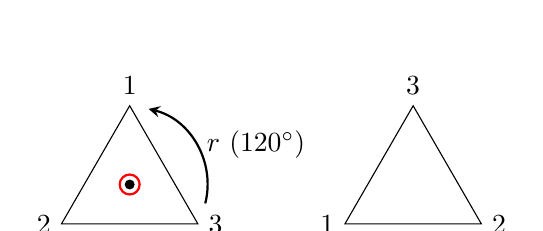
\begin{tikzpicture}[scale=1.2]
            % Original Triangle
            \node[regular polygon, regular polygon sides=3, draw, minimum size=2cm] (A) at (0,0) {};
            \node[above] at (A.corner 1) {1};
            \node[left] at (A.corner 2) {2};
            \node[right] at (A.corner 3) {3};
            
            % Rotation Arrow
            \draw[<-, >=stealth, bend left=45, thick] (0.2, 0.8) to node[right] {$r$ (120$^\circ$)} (0.8, -0.2);
            % Center Point
            \fill (0,0) circle (1.5pt);
            \draw[red, thick] (0,0) circle (3pt);
            % Resulting Triangle
            \begin{scope}[xshift=3cm]
                \node[regular polygon, regular polygon sides=3, draw, minimum size=2cm] (B) at (0,0) {};
                \node[above] at (B.corner 1) {3};
                \node[left] at (B.corner 2) {1};
                \node[right] at (B.corner 3) {2};
            \end{scope}
        \end{tikzpicture}
        \caption{Rotation ($r$)}
    \end{subfigure}
    \hfill
    % 
    \begin{subfigure}[t]{0.45\textwidth}
        \centering
        \begin{tikzpicture}[scale=1.2]
            % Original Triangle
            \node[regular polygon, regular polygon sides=3, draw, minimum size=2cm] (C) at (0,0) {};
            \node[above] at (C.corner 1) {1};
            \node[left] at (C.corner 2) {2};
            \node[right] at (C.corner 3) {3};
            
            % Reflection Line (Vertical)
            \draw[dashed, red] (0, 0.8) -- (0, -0.7) node[below] {$s$};
            
            % Resulting Triangle
            \begin{scope}[xshift=3cm]
                \node[regular polygon, regular polygon sides=3, draw, minimum size=2cm] (D) at (0,0) {};
                \node[above] at (D.corner 1) {1};
                \node[left] at (D.corner 2) {3};
                \node[right] at (D.corner 3) {2};
            \end{scope}
        \end{tikzpicture}
        \caption{Reflection ($s$)}
    \end{subfigure}
    \caption{Symmetry Operations on an Equilateral Triangle $(D_3)$}
\end{figure}


\subsection{Classifications}
We broadly classify symmetry groups into two types:
\begin{enumerate}
    \item \imp[blue]{Discrete Symmetries}: These involve a finite or countable number of operations.
    \begin{enumerate}
        \item \imp[orange]{Point Groups}: Groups of symmetries that leave at least one point of the object fixed in space (e.g., rotations and reflections of a molecule)
        \item \imp[orange]{Permutation Groups}: Groups that describe the swapping of identical parts within a system
    \end{enumerate}
    \item \imp[blue]{Continuous Symmetries}: These involve an infinite number of operations that can be arbitrarily close to one another, typically described by Lie groups.
\end{enumerate}

\subsection{Permutation Group}
A permutation group is defined as a subgroup of a symmetric group $\mathfrak{S}(n)$. An $n$ objects can be arranged in $n!$ ways. Thus the group elements of $\mathfrak{S}(n)$ are the permutations of $n$ objects. 

\smallskip
\noindent\textbf{Example}\\
Let us consider permutations of $3$ objects. Group elements can be written in two--line notation.

\begin{equation*}
\pi_1 =
\begin{pmatrix}
1 & 2 & 3 \\
1 & 2 & 3
\end{pmatrix},
\quad
\pi_2 =
\begin{pmatrix}
1 & 2 & 3 \\
2 & 1 & 3
\end{pmatrix},
\quad
\pi_3 =
\begin{pmatrix}
1 & 2 & 3 \\
1 & 3 & 2
\end{pmatrix}
\end{equation*}

\begin{equation*}
\pi_4 =
\begin{pmatrix}
1 & 2 & 3 \\
3 & 2 & 1
\end{pmatrix},
\quad
\pi_5 =
\begin{pmatrix}
1 & 2 & 3 \\
2 & 3 & 1
\end{pmatrix},
\quad
\pi_6 =
\begin{pmatrix}
1 & 2 & 3 \\
3 & 1 & 2
\end{pmatrix}
\end{equation*}
Note that $3! = 1\times2\times3 = 6$, hence this group contains $6$ elements. Also note that column change does not matter as long as the mapping is preserved.

\subsubsection*{How to read!}
\begin{equation*}
\begin{pmatrix}
1 & 2 & 3 \\ 
2 & 1 & 3
\end{pmatrix}
\quad
\Rightarrow
\quad
\begin{tikzpicture}[baseline=(m.center)]
  \matrix (m) [matrix of math nodes, left delimiter=(, right delimiter=)] {
    2 & 1 & 3 \\
    1 & 2 & 3 \\
  };

  % Annotation for the first row
  \draw[->, blue, thick] (m-1-3.east) -- ++(0.5,0.5) node[right, align=left] {initial \\ state};

  % Annotation for the second row
  \draw[->, blue, thick] (m-2-3.east) -- ++(0.5,-0.5) node[right, align=left] {final \\ state};
\end{tikzpicture}
\end{equation*}

\subsubsection*{Elements and relations}
The identity element is 

\begin{equation*}
\pi_1 \pi_1 =
\begin{pmatrix}
1 & 2 & 3 \\
1 & 2 & 3
\end{pmatrix}
= \pi_1 = e
\end{equation*}
Other elements have the following relations 
\begin{equation*}
\pi_2 \pi_2 =
\begin{pmatrix}
1 & 2 & 3 \\
2 & 1 & 3
\end{pmatrix}
\begin{pmatrix}
2 & 1 & 3 \\
1 & 2 & 3 
\end{pmatrix}
=
\begin{pmatrix}
1 & 2 & 3 \\
1 & 2 & 3
\end{pmatrix}
= \pi_1
\end{equation*}

\begin{equation*}
\pi_2 \pi_5 =
\begin{pmatrix}
1 & 2 & 3 \\
2 & 1 & 3
\end{pmatrix}
\begin{pmatrix}
2 & 1 & 3 \\
3 & 2 & 1
\end{pmatrix}
=
\begin{pmatrix}
1 & 2 & 3 \\
3 & 2 & 1
\end{pmatrix}
= \pi_4
\end{equation*}

\begin{equation*}
\pi_5 \pi_2 =
\begin{pmatrix}
1 & 2 & 3 \\
2 & 3 & 1
\end{pmatrix}
\begin{pmatrix}
2 & 3 & 1 \\
1 & 3 & 2
\end{pmatrix}
=
\begin{pmatrix}
1 & 2 & 3 \\
1 & 3 & 2
\end{pmatrix}
= \pi_3
\end{equation*}

\begin{equation*}
\pi_2 \pi_6 =
\begin{pmatrix}
1 & 2 & 3 \\
2 & 1 & 3
\end{pmatrix}
\begin{pmatrix}
2 & 1 & 3 \\
1 & 3 & 2
\end{pmatrix}
=
\begin{pmatrix}
1 & 2 & 3 \\
1 & 3 & 2
\end{pmatrix}
= \pi_3
\end{equation*}
The permutations $\pi_2$, $\pi_3$, and $\pi_4$ have order $2$, since changing two positions twice returns to the original configuration. They follow these relations $(\pi_2)^{-1}=\pi_2$, $(\pi_3)^{-1}=\pi_3$, $(\pi_4)^{-1}=\pi_4$. 
Also we can show
\begin{equation*}
\pi_5^2 =
\begin{pmatrix}
1 & 2 & 3 \\
2 & 3 & 1
\end{pmatrix}
\begin{pmatrix}
1 & 2 & 3 \\
2 & 3 & 1
\end{pmatrix}
=
\begin{pmatrix}
1 & 2 & 3 \\
3 & 1 & 2
\end{pmatrix}
= \pi_6
\end{equation*}
Similarly,
\begin{equation*}
\pi_6^2 =
\begin{pmatrix}
1 & 2 & 3 \\
3 & 1 & 2
\end{pmatrix}
\begin{pmatrix}
1 & 2 & 3 \\
3 & 1 & 2
\end{pmatrix}
=
\begin{pmatrix}
1 & 2 & 3 \\
2 & 3 & 1
\end{pmatrix}
= \pi_5
\end{equation*}
So, 
\begin{equation*}
    \boxed{(\pi_6)^{-1}=(\pi_6)^2=\pi_5 \qquad (\pi_5)^{-1}=(\pi_5)^2=\pi_6}
\end{equation*}
So, $\pi_5$ and  $\pi_6$ are order $3$ elements

\subsubsection*{Mapping to an Abstruct Symmetry Group}
We can take the group $\mathfrak{S}(3) = \{e, a, b, b^2, ab, ab^2\}$ and identify $\pi_1$ with $e$, $\pi_2$ with $a$, $\pi_5$ with $b$, $\pi_6$ with $b^2$, $\pi_4$ with $ab$ and $\pi_3$ with $ab^2$. So they are isomorphic.

\begin{stkynote}[cyan]{Cayley's Theorem }
    This theorem states that every finite group is isomorphic to a permutation group which is embedded in some symmetric group. In particular, if $|G| = n$, then $G$ is isomorphic to a subgroup of $\mathfrak{S}(3)_n$.

    \begin{proof}
            Let $G$ be a finite group of order $n$. Label the elements of $G$ as $  G = \{ g_1(=e), g_2, \ldots, g_n \}.$ For each element $g \in G$, then define a map
    \[
    \pi_g : G \rightarrow G \quad\text{s.t.}\;  \pi_g(x) = xg \quad \forall x \in G.
    \]
    Since multiplication by $g$ is bijective in a group, $\pi_g$ is a permutation
    of the set $G$. Hence $\pi_g \in \symS_n$.

    In two-line notation this permutation can be written as
    \[\pi_g =
    \begin{pmatrix}
    g_1 & g_2 & \cdots & g_n \\
    g_1 g & g_2 g & \cdots & g_n g
    \end{pmatrix}.\]

    Now define a mapping
    \[
    \phi : G \rightarrow \symS_n \quad \text{s.t.} \;  \phi(g) = \pi_g.
    \]
    
    Let $g,h \in G$. Then for any $x \in G$,
    \[
    \pi_g(\pi_h(x)) = \pi_g(xh) = (xh)g = x(hg).
    \]
    Thus
    \[
    \pi_g \circ \pi_h = \pi_{hg}.
    \]
    Equivalently, $\phi(g)\phi(h) = \phi(gh).$ Hence $\phi$ is a group \imp{homomorphism}.

    Now suppose
    \[
    \phi(g) = \phi(h).
    \]
    Then
    \[
    \pi_g(x) = \pi_h(x) \quad \text{for all } x \in G.
    \]
    Taking $x = e$, $    eg = eh \Rightarrow g = h.$ Thus $\phi$ is \imp{injective}.

    Since $\phi$ is a homomorphism, the image $ \phi(G) = \{ \pi_g : g \in G \}$ is a subgroup of $\symS_n$ (trivial). Because $\phi$ is injective, \imp{$G$ is isomorphic to its image $\phi(G)$}.
    Therefore

    \[
    G \cong \phi(G) \leq \symS_n.
    \]
    Thus every finite group of order $n$ is isomorphic to a subgroup of the
    symmetric group $\symS_n$.
    \[
    \boxed{G \cong \text{a subgroup of } \symS_n}
    \]
    \end{proof}
\end{stkynote}
\subsection{Cycle Structure}
A cycle structure describes the way a permutation in the symmetric group $\symS_n$ partitions the set of n elements into disjoint permutation cycles,. Every permutation can be uniquely factorized into these disjoint cycles.

\subsubsection*{Cycle}
An $r$-cycle (or cyclic permutation of length $r$) is a set of $r$ distinct elements where each element is mapped to the next in the sequence, with the last element mapping back to the first

\begin{enlight}[green]{\bulb}
    \tcblower
    A fundamental property in group theory is that two permutations are conjugate in $\symS_n$ if and only if they have the \imp{identical cycle structure}. 

    \noindent\textbf{Example}: The permutations $(12)(3)$, $(13)(2)$, and $(1)(23)$ all have the same structure (one $2$-cycle and one $1$-cycle) and thus belong to the same conjugacy class.

\end{enlight}

\subsubsection*{Representation}
\begin{equation*}
\pi = \begin{pmatrix} 
1 & 2 & 3 & 4 & 5 & 6 & 7 \\ 
5 & 7 & 3 & 4 & 6 & 1 & 2 
\end{pmatrix} \quad \Rightarrow \quad \pi = \underbrace{(1,5,6)}_{\text{3-cycle}}\underbrace{(2,7)}_{\text{2-cycle}}\underbrace{(3)(4)}_{\text{1-cycle}} \quad \Rightarrow \quad \pi = (1,5,6)(2,7).
\end{equation*}

\begin{enlight}[orange]{\think}
    \tcblower
    How to take quickly take inverse from the matrix representation?
    \[ \pi_4 = \begin{pmatrix} 1 & 2 & 3 \\ 3 & 2 & 1 \end{pmatrix} \overset{R_1 \leftrightarrow R_2}{\longrightarrow} 
    \begin{pmatrix} 3 & 2 & 1 \\ 1 & 2 & 3 \end{pmatrix}  = 
    \begin{pmatrix} 1 & 2 & 3 \\ 3 & 2 & 1 \end{pmatrix} = \pi_4^{-1} = \pi_4
    \]
    How to take inverse from a cycle structure?
    \begin{gather*}
        (1,2,3) = 1 \rightarrow 2 \rightarrow 3 \rightarrow 1 \\
        (1,2,3)^{-1} = 1 \leftarrow 2 \leftarrow 3 \leftarrow 1 \\
        (1,3,2) = (1,2,3)^{-1} = 1 \rightarrow 3 \rightarrow 2
    \end{gather*}
\end{enlight}

\subsubsection*{Multiplication}
We take an example, take $\pi = (1,5,6)(2,7)$ and $\sigma = (3,6)(2,4,5,7)$. We will calculate $\sigma\pi$ using Left-to-Right convention
\begin{gather*}
1 \xrightarrow{\sigma} 1 \xrightarrow{\pi} 5 \implies 1 \to 5 \\
5 \xrightarrow{\sigma} 7 \xrightarrow{\pi} 2 \implies 5 \to 2 \\
2 \xrightarrow{\sigma} 4 \xrightarrow{\pi} 4 \implies 2 \to 4 \\
4 \xrightarrow{\sigma} 5 \xrightarrow{\pi} 6 \implies 4 \to 6 \\
6 \xrightarrow{\sigma} 3 \xrightarrow{\pi} 3 \implies 6 \to 3 \\
3 \xrightarrow{\sigma} 6 \xrightarrow{\pi} 1 \implies 3 \to 1 \\
\end{gather*}
So we have 
\[ \sigma\pi = (1, 5, 2, 4, 6, 3) \]

\newpage
\appendix
\section{Basic Notions from Ring Theory}

A \emph{ring} is a set $R$ equipped with two binary operations, addition and multiplication, such that:

\begin{enumerate}
\item $(R,+)$ is an abelian group,
\item multiplication is associative,
\item multiplication distributes over addition, i.e.
\begin{equation*}
a(b+c)=ab+ac, \qquad (a+b)c=ac+bc.
\end{equation*}
\end{enumerate}

If there exists an element $1 \in R$ satisfying
\begin{equation*}
1a = a1 = a \quad \text{for all } a \in R,
\end{equation*}
then $R$ is called a ring with identity.

\subsection{The Ring \texorpdfstring{$\mathbb{Z}_n$}{Z_n}}

For a fixed integer $n \geq 1$, the set of residue classes modulo $n$,
\begin{equation*}
\mathbb{Z}_n = \{[0],[1],\dots,[n-1]\},
\end{equation*}
forms a finite commutative ring under
\begin{equation*}
[a]+[b]=[a+b], \qquad [a]\cdot[b]=[ab].
\end{equation*}

\subsection{Examples.}

\paragraph{Example 1}
In $\mathbb{Z}_5$,
\begin{equation*}
[2]\cdot[3] = [6] = [1],
\end{equation*}
so every nonzero element has a multiplicative inverse; hence $\mathbb{Z}_5$ is a field.
\paragraph{Example 2}
In $\mathbb{Z}_6$,
\begin{equation*}
[2]\cdot[3] = [6] = [0],
\end{equation*}
so nonzero elements may multiply to zero. Such elements are called zero divisors.

\begin{myquote}[red]
    The ring $\mathbb{Z}_n$ is a field if and only if $n$ is prime.
\end{myquote}

\subsection{Connection with Group Theory}

The additive structure $(\mathbb{Z}_n,+)$ is a finite cyclic group of order $n$ generated by $[1]$. Thus, if an element $r$ in a group satisfies
\begin{equation*}
r^n = e,
\end{equation*}
then
\begin{equation*}
\langle r \rangle \cong (\mathbb{Z}_n,+),
\end{equation*}
and exponent arithmetic is naturally computed modulo $n$.

\section{Modulo Arithmetic and the Structure of \texorpdfstring{$\mathbb{Z}_n$}{Z_n}}

\subsection{Congruence Modulo $n$}

Let $n \in \mathbb{N}$ with $n \geq 1$. For $a,b \in \mathbb{Z}$, we define
\begin{equation*}
a \equiv b \pmod{n}
\end{equation*}

if and only if $n \mid (a-b).$ Equivalently, $a \equiv b \pmod{n}$ if there exists $k \in \mathbb{Z}$ such that $a = b + kn.$ This relation is an equivalence relation on $\mathbb{Z}$.

\subsection{Residue Classes}

For $a \in \mathbb{Z}$, the residue class of $a$ modulo $n$ is defined by
\begin{equation*}
[a] = \{ a + kn \mid k \in \mathbb{Z} \}.
\end{equation*}
The set of all residue classes modulo $n$ is denoted by
\begin{equation*}
\mathbb{Z}_n = \{ [0], [1], \dots, [n-1] \}.
\end{equation*}
Each integer belongs to exactly one residue class.

\subsection{Arithmetic in \texorpdfstring{$\mathbb{Z}_n$}{Z_n}}

Addition and multiplication in $\mathbb{Z}_n$ are defined by
\begin{equation*}
[a] + [b] = [a+b],
\end{equation*}
\begin{equation*}
[a]\cdot[b] = [ab].
\end{equation*}
These operations are well-defined and make $\mathbb{Z}_n$ a commutative ring.

\subsection{Examples}

\paragraph{Example 1.} 
\begin{equation*}
17 \equiv 5 \pmod{12}
\end{equation*}
since
\begin{equation*}
17 - 5 = 12,
\end{equation*}
and $12$ is divisible by $12$.

\paragraph{Example 2.} Arithmetic in $\mathbb{Z}_5$:
\begin{equation*}
[3] + [4] = [7] = [2],
\end{equation*}
\begin{equation*}
[3]\cdot[4] = [12] = [2].
\end{equation*}

\subsection{Algebraic Properties}

If
\begin{equation*}
a \equiv b \pmod{n}
\quad \text{and} \quad
c \equiv d \pmod{n},
\end{equation*}
then
\begin{equation*}
a+c \equiv b+d \pmod{n},
\end{equation*}
\begin{equation*}
ac \equiv bd \pmod{n}.
\end{equation*}

\subsection{Connection with Cyclic Groups}

The additive group $(\mathbb{Z}_n,+)$ is cyclic of order $n$, generated by $[1]$:
\begin{equation*}
\mathbb{Z}_n = \langle [1] \rangle.
\end{equation*}
If $r$ satisfies $r^n = e$, then
\begin{equation*}
\langle r \rangle \cong (\mathbb{Z}_n,+),
\end{equation*}
since
\begin{equation*}
r^a r^b = r^{a+b},
\end{equation*}
with exponents computed modulo $n$.

\subsection{Geometric Interpretation}

Modulo arithmetic is cyclic in nature. For instance, in clock arithmetic (modulo $12$),
\begin{equation*}
10 + 5 \equiv 3 \pmod{12}.
\end{equation*}
Thus, two integers are congruent modulo $n$ precisely when they differ by a multiple of $n$.

\newpage
\section{Algebraic Hierarchies}

Algebraic structures are organised hierarchically according to the number of operations defined on a set and the axioms they satisfy. Each successive level in a hierarchy is obtained by imposing an additional structural property.

\subsection{Structures with One Operation}

Beginning with a set equipped with a single associative operation, we obtain:

\begin{itemize}
\item A \imp{semigroup}: associativity holds.
\item A \imp{monoid}: a semigroup with an identity element.
\item A \imp{group}: a monoid in which every element has an inverse.
\end{itemize}

Thus, each step adds exactly one new requirement:
\begin{equation*}
\text{Semigroup} \;\Rightarrow\; \text{Monoid} \;\Rightarrow\; \text{Group}.
\end{equation*}

\subsection{Structures with Two Operations}

When two operations, addition and multiplication, are introduced, the hierarchy becomes:

\begin{itemize}
\item A \imp{ring}: $(R,+)$ is an \underbar{abelian group}, multiplication is associative, and distributive laws hold.
\item An \imp{integral domain}: a commutative ring with identity and no zero divisors.
\item A \imp{field}: an integral domain in which every nonzero element has a multiplicative inverse.
\end{itemize}

Symbolically,
\begin{equation*}
\text{Ring} \;\Rightarrow\; \text{Integral Domain} \;\Rightarrow\; \text{Field}.
\end{equation*}

Each refinement strengthens the algebraic structure by improving the behaviour of multiplication.

\subsection{Conceptual Perspective}

The hierarchy reflects increasing structural control:

\begin{itemize}
\item Identity provides stability.
\item Inverses provide reversibility.
\item Absence of zero divisors ensures cancellation.
\item Multiplicative inverses allow division.
\end{itemize}

Understanding these layers clarifies the role of structures such as cyclic groups and the ring $\mathbb{Z}_n$ in group-theoretic contexts, where often only part of the available algebraic structure is required.

\section{Special Other Groups}
\subsection{The Quaternion Group $Q$}

The \textit{Quaternion Group} $Q$ is a non-abelian group of order $8$. It provides the group structure of the unit quaternions and plays an important role in both algebra and physics.

\subsubsection*{Definition}

The group is defined as
\begin{equation*}
Q = \{e, s, i, j, k, si, sj, sk\},
\end{equation*}
where $e$ is the identity and $s = -e$. $i,j,k$ are imaginary units, and $s$ is the negative of the identity (often represented as $-1$)

\subsubsection*{Relations}

The elements satisfy the fundamental identities
\begin{equation*}
s^2 = e,
\end{equation*}
\begin{equation*}
i^2 = j^2 = k^2 = ijk = s.
\end{equation*}
The cyclic multiplication rules are
\begin{equation*}
ij = k, \qquad jk = i, \qquad ki = j.
\end{equation*}
The group is non-abelian. For example,
\begin{equation*}
ij = sji \quad (\text{equivalently } ij = -ji).
\end{equation*}
The elements $e$ and $s$ commute with all elements of $Q$.

\subsubsection*{Structure of Subgroups}

A remarkable property of $Q$ is that \emph{every subgroup is normal}.  The non-trivial proper subgroups are $\{e, s\},$ and the three subgroups of order $4$ $\{e, s, i, si\}, \{e, s, j, sj\}, \{e, s, k, sk\}.$

\subsubsection*{Element Orders}

The distribution of element orders in $Q$ is:
\begin{equation*}
|Q| = 8,
\end{equation*}
\begin{equation*}
\text{ord}(s) = 2,
\end{equation*}
\begin{equation*}
\text{ord}(i) = \text{ord}(j) = \text{ord}(k) 
= \text{ord}(si) = \text{ord}(sj) = \text{ord}(sk) = 4.
\end{equation*}

\subsubsection*{Comparison with the Dihedral Group $D_4$}

$Q$ and $D_4$ are the only non-abelian groups of order $8$.  
However, they are not isomorphic because their element order distributions differ. Though, they share the same number of conjugacy classes (five) and even the same character table, they are not isomorphic.

\subsubsection*{Conjugacy Classes}

The conjugacy class decomposition of $Q$ is
\begin{equation*}
Q = \{e\} \cup \{s\} 
\cup \{i, si\} 
\cup \{j, sj\} 
\cup \{k, sk\}.
\end{equation*}
Since $e$ and $s$ commute with all elements, they each form their own conjugacy class.

\subsubsection*{Representation via Pauli Matrices}

A faithful matrix representation is given by
\begin{equation*}
i \mapsto -i\sigma_x, \qquad
j \mapsto -i\sigma_y, \qquad
k \mapsto -i\sigma_z.
\end{equation*}

\subsubsection*{Connection to Rotations}

The algebra of unit quaternions is closely related to the rotation group $SO(3)$. Unit quaternions provide an efficient description of rotations in three-dimensional space.

\subsubsection*{Pseudoreal Representations}

The two-dimensional irreducible representation of $Q$ is \imp{pseudoreal} (or quaternionic). This means the representation is equivalent to its complex conjugate but cannot be brought into a real form by a similarity transformation 

One unique shared property is that the two-dimensional representation of the Quaternion group and the fundamental representation of $SU(2)$ are both pseudoreal (or quaternionic). In the context of $SU(2)$, this is demonstrated by the fact that the Pauli matrices are related to their complex conjugates through the antisymmetric matrix $\sigma_y$ (often denoted as $i\sigma_2$)

\subsubsection*{ Role in SU(2) and Double Covering}
The Quaternion group $Q$ is a finite subgroup of $SU(2)$ (the special unitary group in two dimensions). 
While $SU(2)$ is a continuous Lie group generated by the Pauli matrices, $Q$ forms a discrete subset consisting of the eight elements 
$\{\pm I, \pm i\sigma_x, \pm i\sigma_y, \pm i\sigma_z\}$.
Thus $Q$ can be realised as a subgroup of $SU(2)$ made up of these specific unitary matrices. The group $SU(2)$ is the double cover of the rotation group $SO(3)$, meaning there exists a $2$-to-$1$ homomorphism 
$SU(2) \to SO(3)$. 

As a consequence, a full rotation of $2\pi$ in $SO(3)$ corresponds not to the identity in $SU(2)$, but to the element $-1$. In quaternion notation this element is $s$.

This explains why spin-$\tfrac{1}{2}$ particles acquire a minus sign under a $2\pi$ rotation. 
The quaternion group captures this sign structure algebraically and therefore plays an important role in the representation theory of rotations and in quantum mechanics.

\subsection{Dihedral Group}
The Dihedral Group ($D_n$) is the group of symmetries of a regular $n$-sided polygon in two-dimensional space. It consists of both rotations and reflections, making it a fundamental example in geometric and physical symmetry studies.


\noindent\textbf{Generators} : 
Denoted by $r$ (rotation by $2\pi/n$) and $s$ or $\sigma$ (reflection). \\
\noindent\textbf{Relations}: $r^n = 1$, $s^2 = 1$, $srs = r^{-1}$.

\subsubsection*{Conjugacy Classes of $D_n$}


\textbf{Case 1: $n = 2p+1$ (Odd)} \\
In this case there are $p+2$ conjugacy classes. The decomposition of $D_{2p+1}$ into classes is

\begin{equation*}
\begin{aligned}
D_{2p+1}
&=
\{e\}
\cup
\underbrace{
\{r,r^{2p}\}\cup
\{r^2,r^{2p-1}\}\cup
\cdots\cup
\{r^p,r^{p+1}\}
}_{p\ \text{classes}}
\\
&\qquad\cup
\{s,sr,sr^2,\dots,sr^{2p}\}.
\end{aligned}
\end{equation*}
Here:
\begin{itemize}
\item $\{e\}$ forms one class,
\item the rotations form $p$ classes,
\item all reflections form one single class.
\end{itemize}
Thus the total number of conjugacy classes is
\begin{equation*}
1+p+1=p+2.
\end{equation*}

\noindent\textbf{Case 2: $n=2p$ (Even)} \\
In this case there are $p+3$ conjugacy classes. The decomposition of $D_{2p}$ is
\begin{equation*}
\begin{aligned}
D_{2p}
&=
\{e\}
\cup
\{r^p\}
\cup
\underbrace{
\{r,r^{2p-1}\}\cup
\{r^2,r^{2p-2}\}\cup
\cdots\cup
\{r^{p-1},r^{p+1}\}
}_{p-1\ \text{classes}}
\\
&\qquad\cup
\{s,sr^2,\dots,sr^{2p-2}\}
\cup
\{sr,sr^3,\dots,sr^{2p-1}\}.
\end{aligned}
\end{equation*}
Here:
\begin{itemize}
\item $\{e\}$ and $\{r^p\}$ each form a separate class,
\item the remaining rotations form $p-1$ classes as $r^p = r^{-p}$,
\item reflections split into two distinct classes.
\end{itemize}
Thus the total number of conjugacy classes is
\begin{equation*}
(p+1)+2=p+3.
\end{equation*}

\subsubsection*{Example of $D_3$ (Symmetries of an Equilateral Triangle, Order $6$)}

\begin{itemize}
\item \textbf{Subgroups:}
\begin{itemize}
\item Trivial: $\{e\}$ and $D_3$.
\item Rotation subgroup: $\{e, r, r^2\}$ (Order $3$).
\item Reflection subgroups: $\{e, s\}$, $\{e, sr\}$, $\{e, sr^2\}$ (Each of Order $2$).
\end{itemize}

\item \textbf{Normal Subgroups:}
\begin{itemize}
\item The trivial subgroups $\{e\}$ and $D_3$ itself.
\item The cyclic subgroup of rotations $\{e, r, r^2\}$ is the only non-trivial normal subgroup.
\item The reflection subgroups are \textit{not normal} because conjugating one reflection by a rotation gives a different reflection.
\end{itemize}

\item \textbf{Conjugacy Classes:} $D_3$ has \textbf{three classes}:
\begin{itemize}
\item $\{e\}$
\item The rotations: $\{r, r^2\}$
\item The reflections: $\{s, sr, sr^2\}$
\end{itemize}
\end{itemize}

\subsubsection*{Example: $D_4$ (Symmetries of a Square, Order $8$)}

\begin{itemize}
\item \textbf{Subgroups:} $D_4$ has several subgroups, including the rotation group $C_4$ and various reflection subgroups.

\item \textbf{Normal Subgroups:} 
Unlike $Q_8$, not all subgroups of $D_4$ are normal. 
The normal subgroups include the rotation group $\{e, r, r^2, r^3\}$ and the center $\{e, r^2\}$.

\item \textbf{Conjugacy Classes:} $D_4$ has \textbf{five classes}:
\begin{itemize}
\item $\{e\}$
\item $\{r^2\}$ (The $180^\circ$ rotation)
\item $\{r, r^3\}$ (The $90^\circ$ and $270^\circ$ rotations)
\item $\{\sigma, \sigma r^2\}$ (Reflections across axes through midpoints of sides)
\item $\{\sigma r, \sigma r^3\}$ (Reflections across diagonal axes through vertices)
\end{itemize}
\end{itemize}
\end{document}